\documentclass[11pt,letterpaper]{article}
\usepackage{fontspec}
\setmainfont{texgyrepagella}[Extension=.otf,UprightFont=*-regular,BoldFont=*-bold,ItalicFont=*-italic,BoldItalicFont=*-bolditalic]
\usepackage[bidi=default]{babel}
\babelprovide[import,main]{spanish}
\babelprovide[import]{hebrew}
\babelprovide[import]{ancientgreek}
\babelfont[hebrew]{rm}[Path=fonts/,BoldFont=NotoHebrewSerif-700.ttf,Scale=0.95]{NotoHebrewSerif-400.ttf}
\babelfont[ancientgreek]{rm}[Path=fonts/]{GFSPorson.otf}
\newcommand{\heb}[1]{\mbox{\foreignlanguage{hebrew}{#1}}}
\newcommand{\grc}[1]{\foreignlanguage{ancientgreek}{#1}}
\newcommand{\hebverso}[1]{\par\smallskip{\centering\begin{otherlanguage}{hebrew}\large #1\end{otherlanguage}\par}\smallskip}
\newcommand{\SENOR}{\textsc{Señor}}
\usepackage[margin=2.5cm,headheight=14pt]{geometry}
\usepackage{microtype,ragged2e,booktabs,graphicx,xcolor,csquotes,array}
\usepackage[hidelinks]{hyperref}\usepackage{xurl}\urlstyle{same}
\usepackage[most]{tcolorbox}
\usepackage{tikz}\usetikzlibrary{arrows.meta,positioning,calc,decorations.pathreplacing}
\usepackage{titlesec,fancyhdr}
\definecolor{azul}{HTML}{15437C}\definecolor{azuloscuro}{HTML}{0B1F3A}\definecolor{celeste}{HTML}{5694D6}
\definecolor{dorado}{RGB}{196,154,60}\definecolor{papiro}{RGB}{246,239,220}\definecolor{gris}{RGB}{70,78,96}
\titleformat{\section}{\Large\bfseries\color{azul}}{\thesection.}{0.6em}{}
\titleformat{\subsection}{\large\bfseries\color{azuloscuro}}{\thesubsection}{0.6em}{}
\pagestyle{fancy}\fancyhf{}
\fancyhead[L]{\foreignlanguage{spanish}{\small\itshape\color{gris}La santidad de Dios}}\fancyhead[R]{\foreignlanguage{spanish}{\small\color{gris}\thepage}}
\renewcommand{\headrulewidth}{0.4pt}
\setlength{\parindent}{1.27cm}\linespread{1.15}\setlength{\emergencystretch}{3em}
\newtcolorbox{cita}[1][]{enhanced,colback=azul!6!white,colframe=azul,boxrule=0pt,leftrule=2.5pt,arc=0pt,
  left=8pt,right=8pt,top=5pt,bottom=5pt,before skip=8pt,after skip=8pt,fontupper=\itshape,#1}
\newcommand{\fuente}[1]{\par\hfill{\upshape\bfseries\small\textcolor{azul}{#1}}}
\newtcolorbox{nota}[1][]{enhanced,colback=dorado!10,colframe=dorado!85!azul,boxrule=0.6pt,arc=2pt,
  fonttitle=\bfseries\small,coltitle=azuloscuro,colbacktitle=dorado!30,fontupper=\small,title={#1}}
\newtcolorbox{filologia}[1][]{enhanced,colback=white,colframe=azul!45,boxrule=0.5pt,arc=2pt,
  fonttitle=\bfseries\small,coltitle=white,colbacktitle=azul!80,fontupper=\small,title={Filología: #1}}
\newcommand{\refapa}[1]{\par{\RaggedRight\hangindent=1.27cm\hangafter=1\noindent #1\par}\vspace{4pt}}
\newcommand{\destacar}[1]{\textbf{\textcolor{azul}{#1}}}
\newcolumntype{L}[1]{>{\RaggedRight\arraybackslash}p{#1}}

\title{\color{azul}\bfseries Santo, santo, santo\\[4pt]\large\color{gris}\mdseries La santidad de Dios: la perfección que lo hace sin igual}
\author{}\date{}
\begin{document}
\maketitle\thispagestyle{empty}

\begin{abstract}\noindent
Este capítulo estudia la santidad de Dios desde Isaías 6, donde los serafines la proclaman tres veces. Sostiene que la santidad no es un atributo más entre otros: es la perfección que hace a Dios único, sin igual, y que da a cada uno de sus atributos su carácter divino. El recorrido parte del texto ancla, pasa por la confesión de Ana (``No hay santo como el \SENOR'', 1~S 2:2), analiza la raíz hebrea \heb{קדשׁ}, muestra cómo la santidad califica el poder, la justicia, la fidelidad y la misericordia de Dios, y se detiene en el encuentro de Moisés con la zarza. Luego lee el atributo con Pablo, judío formado en las Escrituras de Israel, que ve la gloria del Santo en el rostro de Jesucristo. Termina con su aplicación a la vida del creyente.
\par\smallskip\noindent\textbf{Palabras clave:} santidad, \emph{qadosh}, Isaías 6, trisagio, Pablo, santificación.\end{abstract}

\begin{nota}[Nota sobre el texto]
Las citas bíblicas son de la Reina-Valera 1960. Donde esta escribe ``Jehová'', aquí se escribe \SENOR, que traduce el tetragrama \heb{יהוה}, leído en la tradición judía como \emph{Adonay}. Cuando el hebreo dice \heb{אֲדֹנָי} (\emph{Adonay}), la RVR1960 escribe ``Señor'' y así se conserva. El hebreo sigue la BHS; el griego, NA28 y la Septuaginta de Rahlfs-Hanhart. En Salmos y Ezequiel se da la numeración española y la hebrea entre corchetes cuando difieren.
\end{nota}

%===================================================================
\section{Texto ancla: Isaías 6:1--8}

\subsection{El año en que murió Uzías}
Isaías fecha su visión por la muerte de un rey: ``en el año que murió el rey Uzías'' (Is 6:1), hacia el 740~a.\,e.\,c. Uzías reinó cincuenta y dos años (2~Cr 26:3) y fue un rey próspero, pero al final de su vida entró al templo para quemar incienso, una tarea reservada a los sacerdotes, y fue herido de lepra hasta su muerte (2~Cr 26:16--21). El rey que quiso entrar en lo santo sin derecho muere; ese mismo año el profeta ve al Rey que está sentado en el trono y que no muere.

\begin{nota}[Precisión]
El contraste entre Uzías, que profanó el santuario, y el Rey santo de Is 6 es una lectura de varios intérpretes (p.~ej., Oswalt, 1986). Isaías solo da la fecha; no hace explícita la comparación.
\end{nota}

\subsection{La visión}
\hebverso{קָדוֹשׁ ׀ קָדוֹשׁ קָדוֹשׁ יְהוָה צְבָאוֹת \\ מְלֹא כָל־הָאָרֶץ כְּבוֹדוֹ}
\begin{cita}En el año que murió el rey Uzías vi yo al Señor sentado sobre un trono alto y sublime, y sus faldas llenaban el templo. Por encima de él había serafines; cada uno tenía seis alas; con dos cubrían sus rostros, con dos cubrían sus pies, y con dos volaban. Y el uno al otro daba voces, diciendo: Santo, santo, santo, \SENOR{} de los ejércitos; toda la tierra está llena de su gloria. Y los quiciales de las puertas se estremecieron con la voz del que clamaba, y la casa se llenó de humo.\fuente{(Is 6:1--4)}\end{cita}

\begin{filologia}[Is 6:1--4]
\begin{tabular}{@{}L{3.2cm}L{1.6cm}L{10cm}@{}}
\heb{אֲדֹנָי} \emph{Adonay} & \heb{אדן} & ``Señor'' (v.~1): título de soberanía, ``mi Señor''. En el v.~3 aparece el nombre propio, \heb{יהוה}. \\[2pt]
\heb{רָם וְנִשָּׂא} \emph{ram venissá} & \heb{רום}, \heb{נשׂא} & ``alto y sublime'': el trono está elevado. Las mismas dos raíces vuelven en Is 52:13 (el Siervo) y 57:15 (Dios). \\[2pt]
\heb{שְׂרָפִים} \emph{serafim} & \heb{שׂרף} & ``los ardientes''; la raíz significa ``quemar''. Son seres que arden y, aun así, se cubren ante Dios. \\[2pt]
\heb{קָדוֹשׁ} \emph{qadosh} & \heb{קדשׁ} & ``santo'': apartado, propio del ámbito de Dios, distinto de lo común (Koehler y Baumgartner, 2001). Repetido tres veces. \\[2pt]
\heb{צְבָאוֹת} \emph{tseva'ot} & \heb{צבא} & ``ejércitos'': las huestes del cielo. Presenta a Dios como Rey y comandante. \\[2pt]
\heb{מְלֹא} \emph{melo} & \heb{מלא} & ``plenitud'': literalmente, ``la plenitud de toda la tierra es su gloria''. \\[2pt]
\heb{כָּבוֹד} \emph{kavod} & \heb{כבד} & ``gloria''; la raíz significa ``ser pesado''. La gloria es el peso de Dios, su santidad hecha visible. \\
\end{tabular}
\end{filologia}

\subsection{¿Por qué tres veces?}
El hebreo intensifica repitiendo. ``La justicia, la justicia seguirás'' (Dt 16:20; \heb{צֶדֶק צֶדֶק}, \emph{tsédeq tsédeq}) significa ``solo la justicia, de verdad la justicia''; dos repeticiones ya expresan intensidad. Tres repeticiones son raras y señalan el grado máximo: ``¡Tierra, tierra, tierra!'' (Jer 22:29); ``A ruina, a ruina, a ruina'' (Ez 21:27 [21:32]). Ningún otro atributo de Dios recibe en la Escritura esta triple aclamación. Los serafines no cantan ``eterno, eterno, eterno'' ni ``poderoso, poderoso, poderoso''. La santidad es lo que el cielo proclama, y lo sigue proclamando:

\begin{cita}y no cesaban día y noche de decir: Santo, santo, santo es el Señor Dios Todopoderoso, el que era, el que es, y el que ha de venir.\fuente{(Ap 4:8)}\end{cita}

\begin{filologia}[Ap 4:8]
\grc{ἅγιος ἅγιος ἅγιος κύριος ὁ θεὸς ὁ παντοκράτωρ}. La LXX de Is 6:3 dice \grc{ἅγιος ἅγιος ἅγιος κύριος σαβαωθ}; Apocalipsis cambia \emph{sabaōth} por \grc{παντοκράτωρ} (\emph{pantokrátōr}, ``Todopoderoso''), la palabra con que la LXX traduce \emph{tseva'ot} en otros libros. \grc{ἅγιος} (\emph{hágios}) es la traducción habitual de \emph{qadosh} en la LXX (Bauer et~al., 2000).
\end{filologia}

\begin{nota}[Precisión]
Desde los Padres de la Iglesia, el ``santo'' triple y el plural ``¿quién irá por nosotros?'' (v.~8) se han leído en clave trinitaria. Es una lectura tradicional; el texto de Isaías no la explicita.
\end{nota}

\subsection{Confesión, expiación y envío}
\begin{cita}Entonces dije: ¡Ay de mí! que soy muerto; porque siendo hombre inmundo de labios, y habitando en medio de pueblo que tiene labios inmundos, han visto mis ojos al Rey, \SENOR{} de los ejércitos. Y voló hacia mí uno de los serafines, teniendo en su mano un carbón encendido, tomado del altar con unas tenazas; y tocando con él sobre mi boca, dijo: He aquí que esto tocó tus labios, y es quitada tu culpa, y limpio tu pecado. Después oí la voz del Señor, que decía: ¿A quién enviaré, y quién irá por nosotros? Entonces respondí yo: Heme aquí, envíame a mí.\fuente{(Is 6:5--8)}\end{cita}

\begin{filologia}[Is 6:5--7]
\begin{tabular}{@{}L{3.2cm}L{1.6cm}L{10cm}@{}}
\heb{אוֹי־לִי} \emph{oy-li} & --- & ``¡Ay de mí!'': fórmula de lamento fúnebre. En el capítulo anterior Isaías pronunció seis ``¡ay!'' sobre Judá (Is 5:8--22); ahora lo dice sobre sí mismo. \\[2pt]
\heb{נִדְמֵיתִי} \emph{nidmeti} & \heb{דמה} & ``soy muerto'' (RVR1960); también puede traducirse ``estoy perdido'' o ``he sido silenciado''. El de labios inmundos queda sin voz ante el trisagio. \\[2pt]
\heb{טְמֵא־שְׂפָתַיִם} \emph{teme sefatayim} & \heb{טמא} & ``inmundo de labios'': lo opuesto a lo santo. El serafín toca justamente los labios. \\[2pt]
\heb{תְּכֻפָּר} \emph{tekuppar} & \heb{כפר} & ``es expiado'' (RVR1960: ``limpio tu pecado''). Es la raíz de \emph{Yom Kippur} y de \heb{כַּפֹּרֶת} (\emph{kapporet}), la tapa del arca o propiciatorio. \\
\end{tabular}
\end{filologia}

El orden del pasaje es parte del mensaje: visión, confesión, expiación y envío. La santidad de Dios primero deja a Isaías sin palabras y luego le devuelve la voz. El mismo fuego que lo condenaría es el que, tomado del altar, quita su culpa. Rudolf Otto (1917/1980) describió la experiencia de lo santo como un misterio que a la vez hace temblar y atrae; Isaías vive las dos cosas: tiembla y luego se ofrece.

\begin{center}
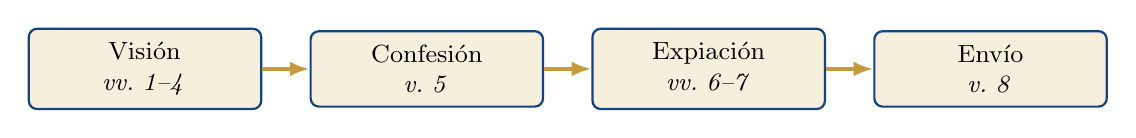
\begin{tikzpicture}[font=\small,node distance=0.6cm,
  b/.style={draw=azul,line width=0.8pt,fill=papiro,rounded corners=3pt,text width=2.6cm,align=center,inner sep=5pt}]
 \node[b] (a) {Visión\\ \emph{vv.~1--4}};
 \node[b,right=of a] (b2) {Confesión\\ \emph{v.~5}};
 \node[b,right=of b2] (c) {Expiación\\ \emph{vv.~6--7}};
 \node[b,right=of c] (d) {Envío\\ \emph{v.~8}};
 \foreach \i/\j in {a/b2,b2/c,c/d}\draw[-{Latex[length=2.5mm]},dorado,line width=1.2pt](\i)--(\j);
\end{tikzpicture}\par
{\footnotesize\color{gris}\textit{Figura 1.} Secuencia de Is 6:1--8. \textit{Nota.} Elaboración propia.}
\end{center}

%===================================================================
\section{Sin igual: ``No hay santo como el \SENOR''}

La santidad es lo que hace a Dios único. Lo dice Ana, madre de Samuel, en la oración que pronuncia cuando entrega al hijo que había pedido (1~S 1:27--2:1):

\hebverso{אֵין־קָדוֹשׁ כַּיהוָה כִּי־אֵין בִּלְתֶּךָ \\ וְאֵין צוּר כֵּאלֹהֵינוּ}
\begin{cita}No hay santo como \SENOR; Porque no hay ninguno fuera de ti, Y no hay refugio como el Dios nuestro.\fuente{(1~S 2:2)}\end{cita}

\begin{filologia}[1~S 2:2]
\begin{tabular}{@{}L{3.2cm}L{1.6cm}L{10cm}@{}}
\heb{אֵין} \emph{eyn} & --- & ``no hay'': niega la existencia. Se repite tres veces en el verso. \\[2pt]
\heb{כַּיהוָה} \emph{ka-Adonay} & --- & ``como el \SENOR'': la partícula \heb{כְּ} introduce la comparación que se niega. \\[2pt]
\heb{בִּלְתֶּךָ} \emph{biltéja} & \heb{בלה} & ``fuera de ti'', ``excepto tú''. \\[2pt]
\heb{צוּר} \emph{tsur} & \heb{צור} & ``roca''; la RVR1960 traduce ``refugio''. La roca es imagen de estabilidad y amparo (Dt 32:4). \\
\end{tabular}
\end{filologia}

El paralelismo del verso iguala dos afirmaciones: ``no hay santo como el \SENOR'' y ``no hay ninguno fuera de ti''. Ser santo y ser sin igual son, en la boca de Ana, la misma cosa. La misma idea aparece en la pregunta que canta Israel junto al mar:

\hebverso{מִי־כָמֹכָה בָּאֵלִם יְהוָה \\ מִי כָּמֹכָה נֶאְדָּר בַּקֹּדֶשׁ}
\begin{cita}¿Quién como tú, oh \SENOR, entre los dioses? ¿Quién como tú, magnífico en santidad, terrible en maravillosas hazañas, hacedor de prodigios?\fuente{(Éx 15:11)}\end{cita}

\begin{filologia}[Éx 15:11]
\heb{מִי כָמֹכָה} (\emph{mi jamoja}), ``¿quién como tú?'', es una pregunta sin respuesta: nadie. \heb{נֶאְדָּר} (\emph{ne'dar}, raíz \heb{אדר}) significa ``majestuoso, glorioso''; \heb{בַּקֹּדֶשׁ} (\emph{baqódesh}), ``en santidad''. Dios es incomparable precisamente en su santidad.
\end{filologia}

Isaías lleva la idea hasta el cosmos. Dios mismo pregunta con quién se le puede comparar, y responde señalando las estrellas:

\hebverso{וְאֶל־מִי תְדַמְּיוּנִי וְאֶשְׁוֶה יֹאמַר קָדוֹשׁ}
\begin{cita}¿A qué, pues, me haréis semejante o me compararéis? dice el Santo. Levantad en alto vuestros ojos, y mirad quién creó estas cosas; él saca y cuenta su ejército; a todas llama por sus nombres; ninguna faltará; tal es la grandeza de su fuerza, y el poder de su dominio.\fuente{(Is 40:25--26)}\end{cita}

\begin{filologia}[Is 40:25]
\heb{דמה} (\emph{damah}) es ``asemejar, comparar''. \heb{קָדוֹשׁ} aparece aquí sin artículo, como nombre propio: ``dice Santo''. Las estrellas, que los pueblos vecinos adoraban, son el ``ejército'' que Dios cuenta y llama por nombre.
\end{filologia}

Por eso la santidad hace a Dios más grande que el universo. Todo lo que existe, desde los serafines hasta las estrellas, está del lado de lo creado. Dios está del otro lado de esa línea, y nada la cruza por sí mismo. Salomón lo dijo al dedicar el templo: ``He aquí que los cielos, los cielos de los cielos, no te pueden contener'' (1~R 8:27).

\begin{center}
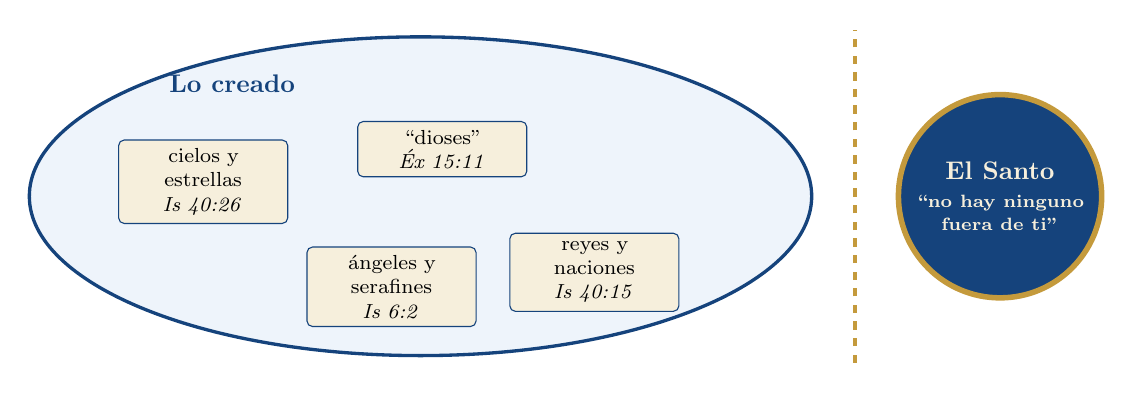
\begin{tikzpicture}[font=\small,scale=0.92,transform shape]
 \draw[azul,line width=1.2pt,fill=celeste!10] (0,0) ellipse (5.4cm and 2.2cm);
 \node[azul,font=\bfseries] at (-2.6,1.55) {Lo creado};
 \foreach \p/\t in {{(-3.0,0.2)}/{cielos y estrellas\\ \emph{Is 40:26}},{(-0.4,-1.25)}/{ángeles y serafines\\ \emph{Is 6:2}},{(2.4,-1.05)}/{reyes y naciones\\ \emph{Is 40:15}},{(0.3,0.65)}/{``dioses''\\ \emph{Éx 15:11}}}
  \node[draw=azul,fill=papiro,rounded corners=2pt,text width=2.1cm,align=center,font=\footnotesize] at \p {\t};
 \draw[dorado,line width=1.4pt,dashed] (6.0,-2.3) -- (6.0,2.3);
 \node[draw=dorado,line width=2pt,fill=azul,text=papiro,circle,minimum size=2.4cm,align=center,font=\bfseries] at (8.0,0) {El Santo\\[-1pt]{\scriptsize ``no hay ninguno}\\[-3pt]{\scriptsize fuera de ti''}};
\end{tikzpicture}\par
{\footnotesize\color{gris}\textit{Figura 2.} La santidad como distinción entre Dios y todo lo creado. \textit{Nota.} Elaboración propia.}
\end{center}

%===================================================================
\section{La palabra: la raíz \heb{קדשׁ}}

\subsection{Familia de palabras}
La raíz \heb{קדשׁ} produce el adjetivo \heb{קָדוֹשׁ} (\emph{qadosh}, ``santo''), el sustantivo \heb{קֹדֶשׁ} (\emph{qódesh}, ``santidad, lo sagrado''), el verbo \heb{קָדַשׁ} (\emph{qadash}, ``ser santo''; en las formas intensivas, ``santificar, consagrar'') y el sustantivo \heb{מִקְדָּשׁ} (\emph{miqdash}, ``santuario''). Su sentido básico es lo \destacar{apartado}: lo que pertenece al ámbito de Dios y queda separado del uso común.

Los usos son concretos antes que abstractos: hay ``tierra santa'' (\heb{אַדְמַת־קֹדֶשׁ}, Éx 3:5), un ``lugar santísimo'' (\heb{קֹדֶשׁ הַקֳּדָשִׁים}, literalmente ``santo de santos'', otro superlativo por repetición), vestiduras santas, aceite santo y un día santo. Isaías llama a Dios \heb{קְדוֹשׁ יִשְׂרָאֵל} (\emph{qedosh Yisra'el}), ``el Santo de Israel'', su título característico.

\begin{nota}[Precisión]
La etimología de \heb{קדשׁ} es discutida. Unos la relacionan con la idea de ``separar'' o ``cortar''; otros, con el acadio \emph{qadāšu}, ``ser puro, limpio'' (Koehler y Baumgartner, 2001). El uso bíblico une las dos ideas: lo santo está apartado y es puro. El número de veces que Isaías usa ``el Santo de Israel'' (cerca de veinticinco) es un conteo aproximado que conviene verificar en la BHS.
\end{nota}

\subsection{Lo santo y lo profano}
\hebverso{וּלֲהַבְדִּיל בֵּין הַקֹּדֶשׁ וּבֵין הַחֹל \\ וּבֵין הַטָּמֵא וּבֵין הַטָּהוֹר}
\begin{cita}para poder discernir entre lo santo y lo profano, y entre lo inmundo y lo limpio.\fuente{(Lv 10:10)}\end{cita}

\begin{filologia}[Lv 10:10]
\heb{הַבְדִּיל} (\emph{havdil}, raíz \heb{בדל}) es ``separar, distinguir''; es el verbo de la creación: ``separó Dios la luz de las tinieblas'' (Gn 1:4). \heb{חֹל} (\emph{jol}) es lo profano o común, lo que no está consagrado. \heb{טָמֵא} (\emph{tame}) es lo inmundo y \heb{טָהוֹר} (\emph{tahor}), lo limpio.
\end{filologia}

El sacerdote debía enseñar a Israel a distinguir. Lo común no es necesariamente malo; simplemente no está apartado para Dios. Lo inmundo, en cambio, no puede acercarse a lo santo. La santidad de Dios ordena toda la vida de Israel alrededor de esa doble distinción.

\subsection{Del hebreo a Pablo}
La Septuaginta traduce casi siempre \emph{qadosh} con \grc{ἅγιος} (\emph{hágios}) y el verbo con \grc{ἁγιάζω} (\emph{hagiázō}). Pablo hereda esas palabras con su carga hebrea y añade dos sustantivos: \grc{ἁγιασμός} (\emph{hagiasmós}, ``santificación'', 1~Ts 4:3, 7; 1~Co 1:30) y \grc{ἁγιωσύνη} (\emph{hagiōsýnē}, ``santidad'' como cualidad), que en el Nuevo Testamento solo aparece en Pablo (Ro 1:4; 2~Co 7:1; 1~Ts 3:13; Bauer et~al., 2000).

\begin{center}
\begin{tikzpicture}[font=\small,node distance=0.8cm,
  b/.style={draw=azul,line width=0.8pt,fill=papiro,rounded corners=3pt,text width=3.4cm,align=center,inner sep=5pt}]
 \node[b] (h) {\textbf{Hebreo}\\ \heb{קָדוֹשׁ} \emph{qadosh}\\ \heb{קֹדֶשׁ} \emph{qódesh}};
 \node[b,right=of h] (l) {\textbf{Septuaginta}\\ \grc{ἅγιος} \emph{hágios}\\ \grc{ἁγιάζω} \emph{hagiázō}};
 \node[b,right=of l] (p) {\textbf{Pablo}\\ \grc{ἁγιασμός} \emph{hagiasmós}\\ \grc{ἁγιωσύνη} \emph{hagiōsýnē}};
 \draw[-{Latex[length=2.5mm]},dorado,line width=1.2pt](h)--(l);
 \draw[-{Latex[length=2.5mm]},dorado,line width=1.2pt](l)--(p);
\end{tikzpicture}\par
{\footnotesize\color{gris}\textit{Figura 3.} El vocabulario de la santidad del hebreo a Pablo. \textit{Nota.} Elaboración propia.}
\end{center}

%===================================================================
\section{Definición}

\begin{tcolorbox}[colback=papiro,colframe=azul,boxrule=1pt,arc=3pt,fonttitle=\bfseries,title=La santidad de Dios]
La santidad es la perfección eterna por la cual Dios es \destacar{absolutamente distinto} de todo lo creado y \destacar{absolutamente puro} de todo mal. Es lo que lo hace único, sin igual (1~S 2:2), y lo que da a cada uno de sus atributos su carácter divino.
\end{tcolorbox}

La definición tiene dos dimensiones y una consecuencia. La primera es la \emph{majestad}: Dios es distinto de toda criatura y nada se le compara (Éx 15:11; Is 40:25). La segunda es la \emph{pureza}: Dios es limpio de todo mal. ``Muy limpio eres de ojos para ver el mal, ni puedes ver el agravio'' (Hab 1:13). La consecuencia sorprende: el Dios que está infinitamente por encima es el mismo que se acerca.

\begin{cita}Porque así dijo el Alto y Sublime, el que habita la eternidad, y cuyo nombre es el Santo: Yo habito en la altura y la santidad, y con el quebrantado y humilde de espíritu, para hacer vivir el espíritu de los humildes, y para vivificar el corazón de los quebrantados.\fuente{(Is 57:15)}\end{cita}

\begin{filologia}[Is 57:15]
\heb{רָם וְנִשָּׂא} (\emph{ram venissá}), ``alto y sublime'', repite las palabras del trono de Is 6:1. \heb{דַּכָּא} (\emph{dakká}) es ``quebrantado, triturado''. El verso pone juntas ``la altura y la santidad'' y la morada con el humilde.
\end{filologia}

\begin{center}\small\renewcommand{\arraystretch}{1.3}
\begin{tabular}{@{}L{3.6cm}L{5.4cm}L{5.4cm}@{}}
\toprule
\textbf{Clasificación} & \textbf{Ubicación} & \textbf{Comentario} \\ \midrule
Grupo & Identidad (¿quién es?) & La santidad define quién es Dios: su Nombre es ``el Santo'' (Is 57:15). \\
Tipo & Incomunicable en su plenitud; comunicable como reflejo & Nadie es santo como él (1~S 2:2), pero manda: ``Santos seréis, porque santo soy yo'' (Lv 19:2). \\
\bottomrule
\end{tabular}\end{center}

\begin{nota}[Precisión]
La clasificación doble (incomunicable en su plenitud, comunicable como reflejo) es una propuesta de este estudio para recoger los dos grupos de textos.
\end{nota}

%===================================================================
\section{La santidad que permea todos sus atributos}

La Escritura no se limita a decir que Dios es poderoso, justo, fiel o misericordioso. Dice que su brazo es \emph{santo}, que su justicia lo muestra \emph{santo}, que jura por su \emph{santidad} y que perdona porque es el \emph{Santo}. La santidad no se suma a los demás atributos: los califica a todos. Por eso el poder de Dios no es arbitrario, su celo no es egoísta y su misericordia no es complicidad con el mal.

\begin{center}
\begin{tikzpicture}[font=\small]
 \node[draw=dorado,line width=2pt,fill=azul,text=papiro,circle,minimum size=2.4cm,font=\large\bfseries,align=center] (c) at (0,0) {SANTO\\[-2pt]{\small\heb{קָדוֹשׁ}}};
 \foreach \ang/\t/\r in {90/{Nombre}/{Sal 111:9},45/{Poder}/{Is 52:10},0/{Justicia}/{Is 5:16},-45/{Fidelidad}/{Sal 89:35},-90/{Celo}/{Jos 24:19},-135/{Misericordia}/{Os 11:9},180/{Sabiduría}/{Pr 9:10},135/{Eternidad}/{Is 57:15}}{
  \node[draw=azul,fill=papiro,rounded corners=3pt,text width=2.1cm,align=center,inner sep=4pt] (n) at (\ang:3.4cm) {\textbf{\textcolor{azul}{\t}}\\ {\footnotesize\r}};
  \draw[dorado,line width=1.1pt] (c) -- (n);}
\end{tikzpicture}\par
{\footnotesize\color{gris}\textit{Figura 4.} La santidad como centro que califica a los demás atributos. \textit{Nota.} Elaboración propia.}
\end{center}

\begin{center}\small\renewcommand{\arraystretch}{1.25}
\begin{tabular}{@{}L{2.2cm}L{6.6cm}L{1.8cm}L{3.6cm}@{}}
\toprule
\textbf{Atributo} & \textbf{Texto (RVR1960)} & \textbf{Cita} & \textbf{Lo que muestra} \\ \midrule
Nombre & ``Santo y temible es su nombre.'' & Sal 111:9 & la santidad es su identidad \\
Eternidad & ``el que habita la eternidad, y cuyo nombre es el Santo'' & Is 57:15 & eterno y santo a la vez \\
Poder & ``\SENOR{} desnudó su santo brazo ante los ojos de todas las naciones'' & Is 52:10 & poder que salva, sin abuso \\
Justicia & ``el Dios Santo será santificado con justicia'' & Is 5:16 & juicio sin corrupción \\
Fidelidad & ``Una vez he jurado por mi santidad, y no mentiré a David.'' & Sal 89:35 [89:36] & jura por lo más alto que es \\
Celo & ``él es Dios santo, y Dios celoso'' & Jos 24:19 & celo sin egoísmo \\
Misericordia & ``porque Dios soy, y no hombre, el Santo en medio de ti'' & Os 11:9 & perdona \emph{porque} es santo \\
Sabiduría & ``el conocimiento del Santísimo es la inteligencia'' & Pr 9:10 & la sabiduría comienza en él \\
Verdad & ``Esto dice el Santo, el Verdadero'' & Ap 3:7 & santo y verdadero (dicho de Cristo) \\
\bottomrule
\end{tabular}\end{center}

Oseas 11:9 merece atención. Israel merecía el juicio, y Dios dice: ``No ejecutaré el ardor de mi ira, ni volveré para destruir a Efraín; porque Dios soy, y no hombre, el Santo en medio de ti''. La razón de la misericordia es la santidad: Dios no reacciona como un hombre ofendido, porque no es hombre.

\begin{filologia}[Os 11:9]
\heb{כִּי אֵל אָנֹכִי וְלֹא־אִישׁ בְּקִרְבְּךָ קָדוֹשׁ}: ``porque Dios (\heb{אֵל}, \emph{El}) soy yo, y no hombre (\heb{אִישׁ}, \emph{ish}); en medio de ti, santo''. La santidad aparece aquí como alteridad: Dios es distinto del hombre incluso en su manera de perdonar.
\end{filologia}

\subsection{La exposición de Pink}
Pink abre su estudio de la santidad con la pregunta de Éx 15:11 y recorre el atributo en cinco movimientos (Pink, 1930/2020). Primero, solo Dios es santo en sí mismo; la criatura lo es solo por derivación. Segundo, su santidad se manifiesta en sus obras, en su ley, que ``a la verdad es santa'' (Ro 7:12), y sobre todo en la cruz, donde Dios no perdonó el pecado ni siquiera cuando lo cargó su Hijo. Tercero, porque es santo, aborrece el pecado. Cuarto, porque es santo, nadie puede ser aceptado por él sobre la base de sus propias obras. Quinto, porque es santo, se le debe adorar con la más profunda reverencia (Sal 89:7 [89:8]; 99:5).

\begin{cita}Exaltad a \SENOR{} nuestro Dios, y postraos ante su santo monte, porque \SENOR{} nuestro Dios es santo.\fuente{(Sal 99:9)}\end{cita}

\begin{filologia}[Sal 99]
El salmo repite como estribillo ``él es santo'' (\heb{קָדוֹשׁ הוּא}, vv.~3 y 5) y cierra con ``santo es el \SENOR{} nuestro Dios'' (v.~9). La forma del salmo reproduce el trisagio: tres veces, en tres estrofas.
\end{filologia}

\begin{nota}[Precisión]
La idea de la santidad como la ``hermosura'' de Dios, que da brillo a todos sus demás atributos, viene de Stephen Charnock (1682/1996), autor puritano al que Pink sigue de cerca. El resumen de Pink en cinco puntos es una paráfrasis de su recorrido, no una cita.
\end{nota}

%===================================================================
\section{Un encuentro en la historia de Israel: Moisés en la zarza}

Moisés lleva cuarenta años como pastor en Madián. Junto a Horeb ve una zarza que arde sin consumirse y se acerca a mirar (Éx 3:1--3). Entonces Dios lo llama por su nombre y lo detiene:

\hebverso{אַל־תִּקְרַב הֲלֹם שַׁל־נְעָלֶיךָ מֵעַל רַגְלֶיךָ \\ כִּי הַמָּקוֹם אֲשֶׁר אַתָּה עוֹמֵד עָלָיו אַדְמַת־קֹדֶשׁ הוּא}
\begin{cita}Y dijo: No te acerques; quita tu calzado de tus pies, porque el lugar en que tú estás, tierra santa es. Y dijo: Yo soy el Dios de tu padre, Dios de Abraham, Dios de Isaac, y Dios de Jacob. Entonces Moisés cubrió su rostro, porque tuvo miedo de mirar a Dios.\fuente{(Éx 3:5--6)}\end{cita}

\begin{filologia}[Éx 3:5]
\begin{tabular}{@{}L{3.2cm}L{1.6cm}L{10cm}@{}}
\heb{אַל־תִּקְרַב} \emph{al-tiqrav} & \heb{קרב} & ``no te acerques''. Es la raíz de \emph{qorbán}, la ofrenda que ``se acerca'' al altar. A Dios solo se llega por el camino que él abre. \\[2pt]
\heb{שַׁל} \emph{shal} & \heb{נשׁל} & ``quita'', ``desata''. Descalzarse era señal de respeto ante un superior y de reconocer que el lugar no es propio. \\[2pt]
\heb{אַדְמַת־קֹדֶשׁ} \emph{admat-qódesh} & \heb{קדשׁ} & ``tierra de santidad'': el hebreo usa el sustantivo en construcción donde el español usa un adjetivo. \\
\end{tabular}
\end{filologia}

La tierra no es santa por sí misma. Era desierto común el día anterior y lo volvería a ser. La hace santa la presencia del Dios santo. La santidad, en primer lugar, no es una cualidad de las cosas sino de Dios, que santifica todo lo que toca.

\begin{nota}[Precisión]
Según un conteo propio, Éx 3:5 es la primera aparición del sustantivo \emph{qódesh} en la Torá; conviene verificarlo en la BHS o en e-Sword. La raíz aparece antes como verbo en Gn 2:3, donde Dios ``santificó'' el séptimo día.
\end{nota}

Los encuentros de Moisés y de Isaías siguen el mismo patrón:

\begin{center}\small\renewcommand{\arraystretch}{1.3}
\begin{tabular}{@{}L{3.0cm}L{5.6cm}L{5.6cm}@{}}
\toprule
& \textbf{Moisés (Éx 3)} & \textbf{Isaías (Is 6)} \\ \midrule
Dios se manifiesta & fuego en la zarza (3:2) & trono, serafines ``ardientes'' y humo (6:1--4) \\
Se declara la santidad & ``tierra santa es'' (3:5) & ``Santo, santo, santo'' (6:3) \\
El hombre se cubre & ``cubrió su rostro'' (3:6) & ``¡Ay de mí!'' (6:5); los serafines cubren su rostro (6:2) \\
Dios se acerca & ``he descendido para librarlos'' (3:8) & el carbón del altar quita la culpa (6:7) \\
Envío & ``Ven, por tanto, ahora, y te enviaré'' (3:10) & ``¿A quién enviaré?''; ``Envíame a mí'' (6:8) \\
\bottomrule
\end{tabular}\end{center}

\begin{nota}[Precisión]
El paralelo es una lectura propia. Los dos relatos comparten la secuencia típica de los relatos de llamado profético: manifestación, objeción o temor, provisión de Dios y envío.
\end{nota}

En los dos casos, la santidad primero aparta al hombre y luego lo envía. El Santo no desciende para destruir, sino para librar.

%===================================================================
\section{La santidad en Cristo, leída con Pablo}

\subsection{Isaías vio su gloria}
El puente entre el trono de Isaías y Jesús lo tiende el evangelio de Juan. Después de citar Is 6:10, el evangelista afirma:

\begin{cita}Isaías dijo esto cuando vio su gloria, y habló acerca de él.\fuente{(Jn 12:41)}\end{cita}

La gloria que llenaba el templo era la gloria de Cristo. Pablo llega al mismo lugar por otro camino. En 2~Corintios 3 compara el rostro de Moisés, que brillaba después de hablar con Dios (Éx 34:29--35), con la gloria del nuevo pacto, y concluye:

\begin{cita}Porque Dios, que mandó que de las tinieblas resplandeciese la luz, es el que resplandeció en nuestros corazones, para iluminación del conocimiento de la gloria de Dios en la faz de Jesucristo.\fuente{(2~Co 4:6)}\end{cita}

\begin{filologia}[2~Co 4:6]
\grc{δόξα} (\emph{dóxa}) es la palabra con que la Septuaginta traduce \heb{כָּבוֹד}. \grc{ἐν προσώπῳ Ἰησοῦ Χριστοῦ} (\emph{en prosōpō Iēsoû Christoû}): ``en el rostro de Jesucristo''. El \emph{kavod} que llena la tierra en Is 6:3 tiene ahora un rostro humano.
\end{filologia}

\begin{nota}[Precisión]
El puente explícito entre Is 6 y Cristo es de Juan, no de Pablo. En 2~Co 4:6 el eco directo es Gn 1:3 (``sea la luz''); la relación con la gloria de Is 6 es un eco posible dentro del tema de la gloria (Hays, 1989).
\end{nota}

\subsection{``Según el Espíritu de santidad''}
Pablo presenta su evangelio con una fórmula de sabor hebreo:

\begin{cita}que fue declarado Hijo de Dios con poder, según el Espíritu de santidad, por la resurrección de entre los muertos.\fuente{(Ro 1:4)}\end{cita}

\begin{filologia}[Ro 1:4]
\grc{κατὰ πνεῦμα ἁγιωσύνης} (\emph{katà pneûma hagiōsýnēs}), ``según el espíritu de santidad''. Es un hebraísmo: reproduce la construcción de \heb{רוּחַ קָדְשְׁךָ} (\emph{rúaj qodshéja}, ``tu santo espíritu'', literalmente ``espíritu de tu santidad'', Sal 51:11 [51:13]; Is 63:10--11). \grc{ἁγιωσύνη} es un sustantivo de cualidad que en el Nuevo Testamento solo usa Pablo.
\end{filologia}

Pablo, judío formado en las Escrituras de Israel, usa una expresión de los salmos para decir quién es Jesús: el Mesías resucitado pertenece a la esfera de la santidad de Dios.

\begin{nota}[Precisión]
Se discute si ``Espíritu de santidad'' designa al Espíritu Santo o la naturaleza espiritual de Cristo en contraste con ``según la carne'' (v.~3). Moo (1996) se inclina por el Espíritu Santo; Dunn (1998) subraya el contraste entre las dos esferas de la existencia del Hijo.
\end{nota}

\subsection{El carbón del altar y la cruz}
En Is 6:7 el pecado de Isaías ``es expiado'' (\heb{תְּכֻפָּר}) con un carbón tomado del altar. Pablo describe la cruz con el vocabulario del mismo altar:

\begin{cita}por cuanto todos pecaron, y están destituidos de la gloria de Dios, siendo justificados gratuitamente por su gracia, mediante la redención que es en Cristo Jesús, a quien Dios puso como propiciación por medio de la fe en su sangre, para manifestar su justicia, a causa de haber pasado por alto, en su paciencia, los pecados pasados, con la mira de manifestar en este tiempo su justicia, a fin de que él sea el justo, y el que justifica al que es de la fe de Jesús.\fuente{(Ro 3:23--26)}\end{cita}

\begin{filologia}[Ro 3:25]
\grc{ἱλαστήριον} (\emph{hilastērion}), ``propiciación'' o ``propiciatorio'', es la palabra con que la Septuaginta traduce \heb{כַּפֹּרֶת} (\emph{kapporet}), la tapa del arca donde se rociaba la sangre en el Día de la Expiación (Éx 25:17; Lv 16:14--15). \emph{Kapporet} y \emph{tekuppar} (Is 6:7) comparten la raíz \heb{כפר}. Notar también ``destituidos de la gloria'' (\grc{δόξα}, v.~23): lo que el pecador pierde es justamente el \emph{kavod} que llena la tierra en Is 6:3.
\end{filologia}

\begin{center}
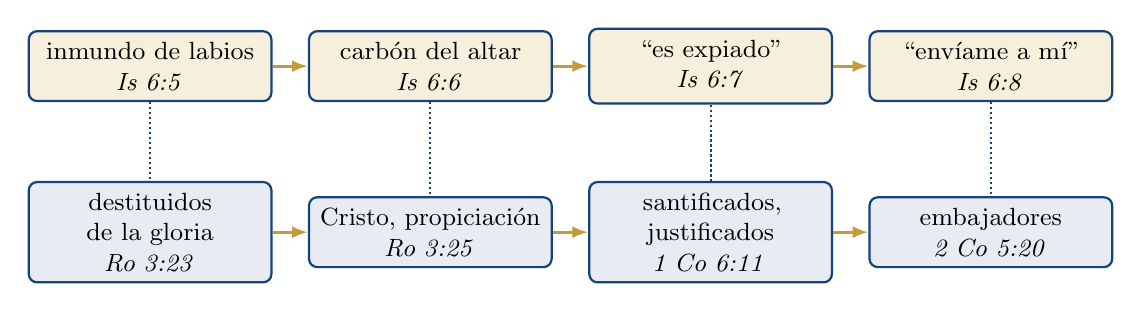
\begin{tikzpicture}[font=\small,node distance=0.45cm,
  b/.style={draw=azul,line width=0.8pt,fill=papiro,rounded corners=3pt,text width=2.8cm,align=center,inner sep=4pt}]
 \node[b] (i1) {inmundo de labios\\ \emph{Is 6:5}};
 \node[b,right=of i1] (i2) {carbón del altar\\ \emph{Is 6:6}};
 \node[b,right=of i2] (i3) {``es expiado''\\ \emph{Is 6:7}};
 \node[b,right=of i3] (i4) {``envíame a mí''\\ \emph{Is 6:8}};
 \node[b,below=1.0cm of i1,fill=azul!10] (p1) {destituidos de la gloria\\ \emph{Ro 3:23}};
 \node[b,right=of p1,fill=azul!10] (p2) {Cristo, propiciación\\ \emph{Ro 3:25}};
 \node[b,right=of p2,fill=azul!10] (p3) {santificados, justificados\\ \emph{1~Co 6:11}};
 \node[b,right=of p3,fill=azul!10] (p4) {embajadores\\ \emph{2~Co 5:20}};
 \foreach \a/\b in {i1/i2,i2/i3,i3/i4,p1/p2,p2/p3,p3/p4}\draw[-{Latex[length=2mm]},dorado,line width=1pt](\a)--(\b);
 \foreach \n in {1,2,3,4}\draw[densely dotted,azul,line width=0.8pt](i\n)--(p\n);
\end{tikzpicture}\par
{\footnotesize\color{gris}\textit{Figura 5.} La secuencia de Isaías 6 y su correspondencia en Pablo. \textit{Nota.} Elaboración propia.}
\end{center}

En la cruz se resuelve la tensión que Isaías sintió en el templo. La santidad de Dios no puede pasar por alto el pecado; si lo hiciera, dejaría de ser justo. En Cristo, Dios es ``el justo, y el que justifica'': la santidad se satisface y el pecador es limpiado.

\begin{nota}[Precisión]
La correspondencia entre el carbón de Is 6 y la cruz es tipológica. Pablo no cita Is 6 en Romanos 3; el vínculo es la raíz \heb{כפר} y el tema común del altar y la expiación.
\end{nota}

\subsection{Cristo, nuestra santificación}
Para Pablo la santidad del creyente no comienza como logro, sino como don:

\begin{cita}Mas por él estáis vosotros en Cristo Jesús, el cual nos ha sido hecho por Dios sabiduría, justificación, santificación y redención, para que, como está escrito: El que se gloría, gloríese en el Señor.\fuente{(1~Co 1:30--31)}\end{cita}

\begin{filologia}[1~Co 1:30]
\grc{ἁγιασμός} (\emph{hagiasmós}): ``santificación'', tanto el estado de estar apartado para Dios como el proceso de vivir de acuerdo con ello (Bauer et~al., 2000). El v.~31 cita Jer 9:24, el versículo que une toda esta obra: gloriarse en conocer al Señor.
\end{filologia}

\begin{cita}Y esto erais algunos; mas ya habéis sido lavados, ya habéis sido santificados, ya habéis sido justificados en el nombre del Señor Jesús, y por el Espíritu de nuestro Dios.\fuente{(1~Co 6:11)}\end{cita}

\begin{filologia}[1~Co 6:11]
\grc{ἡγιάσθητε} (\emph{hēgiásthēte}), ``fuisteis santificados'', está en aoristo pasivo: un hecho ya cumplido y realizado por Dios. La santificación aparece aquí junto al lavamiento y la justificación como obra pasada.
\end{filologia}

Lo que Isaías recibió en los labios, el creyente lo recibe en Cristo. Por eso Pablo puede llamar ``santos'' a los corintios (1~Co 1:2) al mismo tiempo que corrige sus pecados: son santos porque pertenecen al Santo, y deben llegar a ser lo que ya son. La misma idea aparece en Colosenses:

\begin{cita}en su cuerpo de carne, por medio de la muerte, para presentaros santos y sin mancha e irreprensibles delante de él.\fuente{(Col 1:22)}\end{cita}

\begin{nota}[Precisión]
La autoría paulina de Colosenses es discutida. La enseñanza de Col 1:22 tiene respaldo en cartas indiscutidas: 1~Co 6:11 y 1~Ts 3:13.
\end{nota}

\subsection{La plenitud santa habita en Cristo}
La tesis de esta obra encuentra aquí su lugar: ``en él habita corporalmente toda la plenitud de la Deidad'' (Col 2:9). La santidad que los serafines proclaman está entera en Cristo, a quien Pedro llama ``el Santo y el Justo'' (Hch 3:14). En él, el Dios que Isaías no podía mirar sin decir ``¡Ay de mí!'' se deja ver, y el fuego que quema se convierte en perdón.

%===================================================================
\section{Aplicación: vivir ante el Dios santo}

\hebverso{קְדֹשִׁים תִּהְיוּ כִּי קָדוֹשׁ אֲנִי יְהוָה אֱלֹהֵיכֶם}
\begin{cita}Habla a toda la congregación de los hijos de Israel, y diles: Santos seréis, porque santo soy yo \SENOR{} vuestro Dios.\fuente{(Lv 19:2)}\end{cita}

\begin{filologia}[Lv 19:2]
\heb{תִּהְיוּ} (\emph{tihyú}), ``seréis'', es a la vez mandato y promesa. \heb{כִּי} (\emph{ki}), ``porque'', da el fundamento: la santidad de Israel deriva de la de Dios. Pedro cita este verso en 1~P 1:16.
\end{filologia}

La santidad de Dios no es solo una doctrina para entender; es una realidad ante la cual se vive. El texto ancla y los demás pasajes sugieren cinco respuestas:

\begin{enumerate}
\item \textbf{Adorar con reverencia.} Moisés se quitó el calzado y los serafines se cubren el rostro (Éx 3:5; Is 6:2). La adoración no es un trato casual con Dios. ¿Qué ``tierra santa'' pisamos cada domingo sin darnos cuenta?
\item \textbf{Confesar.} Ante el Santo, Isaías no se comparó con sus vecinos: se vio a sí mismo (Is 6:5). La santidad de Dios es la única medida verdadera de nuestra condición.
\item \textbf{Recibir la santidad como don.} El carbón vino del altar, no de Isaías. Cristo nos ha sido hecho santificación (1~Co 1:30; 6:11). La vida santa empieza recibiendo, no produciendo.
\item \textbf{Vivir apartados.} ``Pues no nos ha llamado Dios a inmundicia, sino a santificación'' (1~Ts 4:7). Esto incluye el cuerpo, que Pablo pide presentar ``en sacrificio vivo, santo, agradable a Dios'' (Ro 12:1).
\item \textbf{Responder al envío.} El que ha sido limpiado escucha la pregunta ``¿A quién enviaré?'' y responde ``Heme aquí'' (Is 6:8). Pablo lo dice así: ``somos embajadores en nombre de Cristo'' (2~Co 5:20).
\end{enumerate}

\begin{cita}sino, como aquel que os llamó es santo, sed también vosotros santos en toda vuestra manera de vivir; porque escrito está: Sed santos, porque yo soy santo.\fuente{(1~P 1:15--16)}\end{cita}

%===================================================================
\section{Síntesis}

\begin{tcolorbox}[colback=papiro,colframe=azul,boxrule=1pt,arc=3pt]
Dios es santo: absolutamente distinto de todo lo creado y puro de todo mal. ``No hay santo como el \SENOR; porque no hay ninguno fuera de ti'' (1~S 2:2). Por eso el cielo no canta ``eterno'' ni ``poderoso'' tres veces, sino ``Santo, santo, santo'' (Is 6:3; Ap 4:8). Su santidad califica cada atributo: su brazo es santo, su justicia lo muestra santo, jura por su santidad y perdona porque es ``Dios y no hombre'' (Os 11:9). El trono que vio Isaías es el de Cristo (Jn 12:41); la gloria de Dios brilla en su rostro (2~Co 4:6); en él habita toda la plenitud (Col 2:9), y él nos ha sido hecho santificación (1~Co 1:30).
\end{tcolorbox}

\begin{center}\small\renewcommand{\arraystretch}{1.3}
\begin{tabular}{@{}L{3.0cm}L{11.4cm}@{}}
\toprule
\textbf{Mirada} & \textbf{Aporte al atributo} \\ \midrule
Hebrea & \emph{qadosh}: lo apartado; la triple aclamación; la pregunta ``¿quién como tú?''; la tierra santa de la zarza; la santidad como alteridad que perdona (Os 11:9). \\
Pink & Solo Dios es santo en sí mismo; aborrece el pecado; su santidad se ve en la ley y en la cruz; exige reverencia. \\
Paulina & El Mesías declarado Hijo ``según el Espíritu de santidad''; la gloria del Santo en el rostro de Cristo; la expiación en la cruz; Cristo, nuestra santificación. \\
\bottomrule
\end{tabular}\end{center}

%===================================================================
\section*{Glosario}
\begin{description}\setlength{\itemsep}{2pt}
\item[\emph{Adonay}] (\heb{אֲדֹנָי}). ``Señor''. Título de soberanía; también la lectura judía del tetragrama.
\item[\emph{Hagiasmós}] (\grc{ἁγιασμός}). Santificación: estado y proceso de ser apartado para Dios.
\item[\emph{Hagiōsýnē}] (\grc{ἁγιωσύνη}). Santidad como cualidad. En el Nuevo Testamento, solo en Pablo.
\item[\emph{Hilastērion}] (\grc{ἱλαστήριον}). Propiciatorio o propiciación (Ro 3:25); en la Septuaginta, la tapa del arca.
\item[\emph{Jol}] (\heb{חֹל}). Lo profano o común; lo que no está consagrado.
\item[\emph{Kapporet}] (\heb{כַּפֹּרֶת}). Tapa del arca del pacto, el propiciatorio.
\item[\emph{Kavod}] (\heb{כָּבוֹד}). Gloria; de una raíz que significa ``ser pesado''.
\item[\emph{Kipper}] (\heb{כִּפֶּר}). Expiar, cubrir la culpa.
\item[\emph{Qadosh}] (\heb{קָדוֹשׁ}). Santo, apartado para Dios.
\item[\emph{Qódesh}] (\heb{קֹדֶשׁ}). Santidad; lo sagrado.
\item[\emph{Serafim}] (\heb{שְׂרָפִים}). ``Los ardientes'', seres celestiales de Is 6:2.
\item[Tetragrama] (\heb{יהוה}). El nombre propio de Dios; en esta obra, \SENOR.
\item[Trisagio] La triple aclamación ``Santo, santo, santo'' (Is 6:3; Ap 4:8).
\item[\emph{Tseva'ot}] (\heb{צְבָאוֹת}). ``Ejércitos''; las huestes del cielo.
\item[\emph{Tsur}] (\heb{צוּר}). Roca; imagen de estabilidad y amparo (1~S 2:2).
\end{description}

\section*{Referencias}
\refapa{Bauer, W., Danker, F.~W., Arndt, W.~F., \& Gingrich, F.~W. (2000). \emph{A Greek-English lexicon of the New Testament and other early Christian literature} (3.ª ed.). University of Chicago Press.}
\refapa{\emph{Biblia Reina-Valera 1960}. (1960). Sociedades Bíblicas en América Latina.}
\refapa{Charnock, S. (1996). \emph{The existence and attributes of God} (Vols. 1--2). Baker Books. (Obra original publicada en 1682)}
\refapa{Dunn, J.~D.~G. (1998). \emph{The theology of Paul the apostle}. Eerdmans.}
\refapa{Elliger, K., \& Rudolph, W. (Eds.). (1997). \emph{Biblia Hebraica Stuttgartensia} (5.ª ed.). Deutsche Bibelgesellschaft.}
\refapa{Hays, R.~B. (1989). \emph{Echoes of Scripture in the letters of Paul}. Yale University Press.}
\refapa{Koehler, L., \& Baumgartner, W. (2001). \emph{The Hebrew and Aramaic lexicon of the Old Testament} (M.~E.~J. Richardson, Trad.; Ed. de estudio). Brill.}
\refapa{Moo, D.~J. (1996). \emph{The epistle to the Romans}. Eerdmans.}
\refapa{Nestle, E., \& Aland, K. (2012). \emph{Novum Testamentum Graece} (28.ª ed.). Deutsche Bibelgesellschaft.}
\refapa{Oswalt, J.~N. (1986). \emph{The book of Isaiah: Chapters 1--39}. Eerdmans.}
\refapa{Otto, R. (1980). \emph{Lo santo: Lo racional y lo irracional en la idea de Dios} (F. Vela, Trad.). Alianza Editorial. (Obra original publicada en 1917)}
\refapa{Pink, A.~W. (2020). \emph{Los atributos de Dios}. Chapel Library. (Obra original publicada en 1930)}
\refapa{Rahlfs, A., \& Hanhart, R. (Eds.). (2006). \emph{Septuaginta} (Ed. rev.). Deutsche Bibelgesellschaft.}

\end{document}
